% ============================================================================
% DSD 2026 — Comprehensive Integration Testing Report
% Limb Motion Recognition & Rehabilitation Training Platform
% UTAD × Jilin University
% ============================================================================
\documentclass[aspectratio=169,utf8,11pt]{beamer}
\usepackage{ctex}
\usepackage{booktabs}
\usepackage{colortbl}
\usepackage{xcolor}
\usepackage{tikz}
\usetikzlibrary{positioning}
\usepackage{multirow}
\usepackage{array}
\usepackage{listings}

% ── Theme ─────────────────────────────────────────────────────────────
\usetheme{CambridgeUS}
\usecolortheme{dolphin}
\setbeamertemplate{navigation symbols}{}
\setbeamertemplate{footline}[frame number]
\setbeamercolor{frametitle}{bg=blue!30!black,fg=white}
\setbeamercolor{title}{bg=blue!50!black,fg=white}

% ── Colors ───────────────────────────────────────────────────────────
\definecolor{passgreen}{RGB}{0,130,0}
\definecolor{failred}{RGB}{200,30,30}
\definecolor{warnyel}{RGB}{200,140,0}
\definecolor{infoblue}{RGB}{30,80,180}
\definecolor{bugred}{RGB}{180,20,20}

% ── Commands ──────────────────────────────────────────────────────────
\newcommand{\pass}[1]{\textcolor{passgreen}{\textbf{#1}}}
\newcommand{\fail}[1]{\textcolor{failred}{\textbf{#1}}}
\newcommand{\warn}[1]{\textcolor{warnyel}{\textbf{#1}}}
\newcommand{\bug}[1]{\textcolor{bugred}{\textbf{#1}}}

% ── Title ────────────────────────────────────────────────────────────
\title[DSD 2026 Integration Test]{Limb Motion Training Platform\\\normalsize Integration Test Report}
\subtitle{DSD 2025--2026 · UTAD $\times$ Jilin University}
\author{S1 -- Derui Tang}
\institute{4-Module Collaborative Integration Verification}
\date{June 9, 2026}

\begin{document}

% ============================================================================
% TITLE
% ============================================================================
\begin{frame}[plain]
  \titlepage
  \begin{center}

    \vspace{0.8cm}
    {\footnotesize GitHub Repository: \textcolor{blue}{\url{https://github.com/Dcukducker/DSD2026-integration-test}}}
  \end{center}
\end{frame}

% ============================================================================
% Test Methodology
% ============================================================================
\begin{frame}{Test Methodology}
  \begin{alertblock}{Core Testing Strategy}
    \small
    \begin{itemize}
      \item \textbf{Integration:} Big-Bang — all modules integrated simultaneously and tested as a unified system
      \item \textbf{Type:} Black-Box — verify external behavior via interfaces, not internal logic
      \item \textbf{Focus:} Inter-module API connectivity \& data pipeline integrity over module internals
      \item \textbf{Scope:} Cross-module HTTP APIs, data serialization/deserialization, end-to-end data flows
    \end{itemize}
  \end{alertblock}

  \vspace{0.15cm}
  \begin{block}{Code Version Notes}
    \small
    \begin{itemize}
      \item Based on code submitted to each team's branch before \textbf{June 7, 2026}
      \item Corresponds to \textbf{Phase 1 requirements} — core business processes \& basic interfaces
      \item Code modified after June 7 is \textbf{not included} — development still in progress
      \item Results reflect integration status as of June 7
      \item Helped by LLM Agents for test script generation, debugging, and documentation
    \end{itemize}
    \vspace{0.15cm}
  \end{block}
\end{frame}

% ============================================================================
% OUTLINE
% ============================================================================
\begin{frame}{Outline}
  \tableofcontents[hideallsubsections]
\end{frame}

% ============================================================================
\section{Project Background \& Architecture}
% ============================================================================

\begin{frame}{Project Overview: 4-Module System}
  \begin{columns}[T]
    \begin{column}{0.55\textwidth}
      \begin{table}[h]
        \small
        \rowcolors{2}{gray!10}{white}
        \begin{tabular}{lll}
          \toprule
          \textbf{Module} & \textbf{Tech Stack} & \textbf{Port} \\
          \midrule
          App (S1+S2+M1) & Python Flask & 5000 \\
          V2 Backend & Node.js Express & 3000 \\
          M2 Clinical Web & React+Vite & 5173 \\
          V1 AI Engine & Python Batch & --- \\
          \bottomrule
        \end{tabular}
      \end{table}
    \end{column}
    \begin{column}{0.45\textwidth}
      \begin{block}{Key Scale Metrics}
        \begin{itemize}
          \item V2 Backend \textbf{40+} REST endpoints
          \item Database \textbf{10} tables
          \item Cross-module interfaces \textbf{6} layers
          \item Involving \textbf{60+} API calls
          \item Source code \textbf{11} hardcoded fixes
        \end{itemize}
      \end{block}
    \end{column}
  \end{columns}

  \vspace{0.3cm}
  \begin{center}
    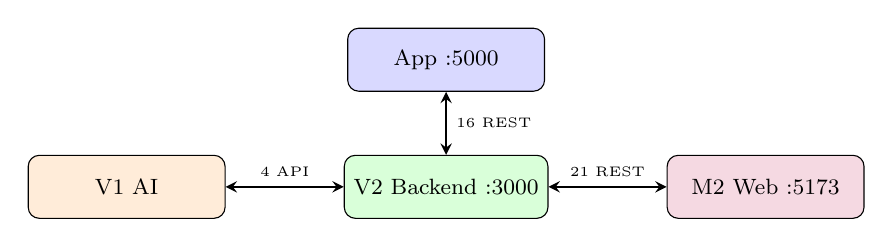
\begin{tikzpicture}[node distance=1.5cm,
      box/.style={rectangle,draw,rounded corners,minimum width=2.5cm,minimum height=0.8cm,align=center,font=\footnotesize},
      arr/.style={->,>=stealth,thick}]
      \node[box,fill=blue!15] (app) {App :5000};
      \node[box,fill=green!15,below=0.8cm of app] (v2) {V2 Backend :3000};
      \node[box,fill=orange!15,left=1.5cm of v2] (v1) {V1 AI};
      \node[box,fill=purple!15,right=1.5cm of v2] (m2) {M2 Web :5173};
      \draw[arr,<->] (app) -- (v2) node[midway,right,font=\tiny] {16 REST};
      \draw[arr,<->] (v1) -- (v2) node[midway,above,font=\tiny] {4 API};
      \draw[arr,<->] (m2) -- (v2) node[midway,above,font=\tiny] {21 REST};
    \end{tikzpicture}
  \end{center}
\end{frame}

\begin{frame}{Pre-Integration Environment \& Blockers}
  \begin{columns}[T]
    \begin{column}{0.45\textwidth}
      \textbf{Branch per Module}
      \begin{table}[h]
        \tiny
        \rowcolors{2}{gray!10}{white}
        \begin{tabular}{ll}
          \toprule
          \textbf{Repository} & \textbf{Branch} \\
          \midrule
          DSD2026-app-windows & feature/recording-upload-cancel \\
          dsd2026-teamv2 & joaolima \\
          project-main-web & main \\
          v1-motion-standard-curves & main \\
          \bottomrule
        \end{tabular}
      \end{table}
    \end{column}
    \begin{column}{0.55\textwidth}
      \begin{alertblock}{Integration Blockers Discovered}
        \begin{enumerate}
          \item \textbf{11 instances} of hardcoded remote URL \texttt{113.44.220.94}
          \item M2 Clinical Web fully mocked data
          \item No unified environment configuration mechanism
          \item No integration test scripts
          \item No automated startup scripts
        \end{enumerate}
      \end{alertblock}
    \end{column}
  \end{columns}

  \begin{block}{Blocker Resolution Effort}
    \begin{itemize}
      \item Modified source files: \textbf{11} (Python×5 + TypeScript×6 + 1 new)
      \item New config/script files: \textbf{7} (.env×3 + scripts×4, later expanded to 9)
      \item All changed to environment variables, defaulting to \texttt{localhost:3000}
    \end{itemize}
  \end{block}
\end{frame}

% ============================================================================
\section{Test System Design}
% ============================================================================

\begin{frame}{Test Architecture: 6-Layer Coverage}
  \begin{center}
    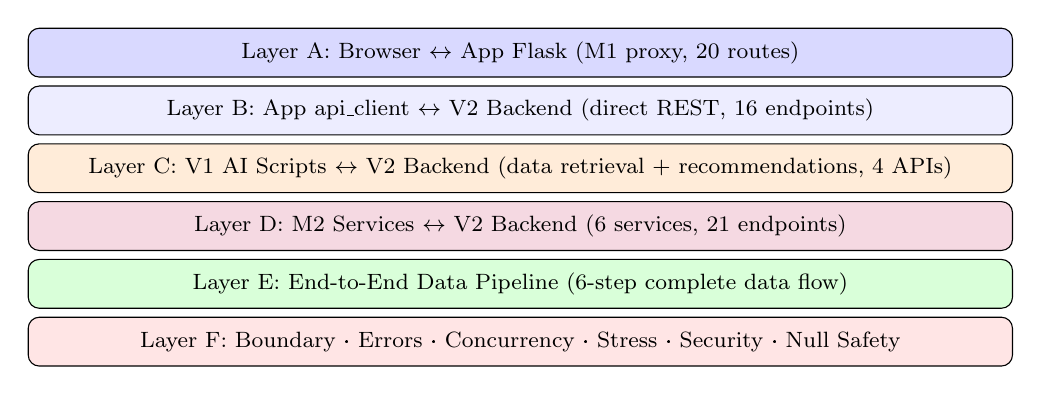
\begin{tikzpicture}[
      layer/.style={rectangle,draw,rounded corners,minimum width=12.5cm,minimum height=0.62cm,align=center,font=\footnotesize}]
      \node[layer,fill=blue!15] (A) {Layer A: Browser $\leftrightarrow$ App Flask (M1 proxy, 20 routes)};
      \node[layer,fill=blue!7,below=0.10cm of A] (B) {Layer B: App api\_client $\leftrightarrow$ V2 Backend (direct REST, 16 endpoints)};
      \node[layer,fill=orange!15,below=0.10cm of B] (C) {Layer C: V1 AI Scripts $\leftrightarrow$ V2 Backend (data retrieval + recommendations, 4 APIs)};
      \node[layer,fill=purple!15,below=0.10cm of C] (D) {Layer D: M2 Services $\leftrightarrow$ V2 Backend (6 services, 21 endpoints)};
      \node[layer,fill=green!15,below=0.10cm of D] (E) {Layer E: End-to-End Data Pipeline (6-step complete data flow)};
      \node[layer,fill=red!10,below=0.10cm of E] (F) {Layer F: Boundary · Errors · Concurrency · Stress · Security · Null Safety};
    \end{tikzpicture}
  \end{center}
  \vspace{0.15cm}
  \begin{block}{Design Philosophy}
    \footnotesize Bottom-up layer-by-layer validation: API calls $\rightarrow$ point-to-point interfaces $\rightarrow$ complete pipelines $\rightarrow$ exception scenarios.\\
    Each layer must pass before proceeding to the next; fully automated execution with direct PASS/FAIL output.
  \end{block}
\end{frame}

\begin{frame}{Test Script Matrix: 6 Scripts × 166 Items}
  \vspace{0.2cm}
  \begin{table}[h]
    \centering
    \renewcommand{\arraystretch}{1.4}
    \footnotesize
    \begin{tabular}{p{3.0cm}p{3.1cm}p{1.3cm}p{1.6cm}p{2.0cm}}
      \toprule
      \textbf{Script File} & \textbf{Test Type} & \textbf{Items} & \textbf{Duration} & \textbf{Result} \\
      \midrule
      \texttt{smoke\_test.ps1} & Core API Quick Connectivity & 14 & $\sim$1 min & \cellcolor{green!15}100\% PASS \\
      \texttt{integration\_test.ps1} & 6-Layer Full Interface Coverage & 62 & $\sim$2 min & \cellcolor{green!15}100\% PASS \\
      \texttt{pipeline\_test.ps1} & 3 Use Case Data Pipelines & 26 & $\sim$3 min & \cellcolor{green!15}100\% PASS \\
      \texttt{scenario\_test.ps1} & Concurrency/Stress/Boundary & 17 & $\sim$1 min & \cellcolor{green!15}100\% PASS \\
      \texttt{bug\_hunt.ps1} & Security \& Defect Detection & 13 & $\sim$1 min & Found \bug{10 bugs} \\
      \texttt{null\_safety.ps1} & Null/Missing Field Safety & 34 & $\sim$1 min & \cellcolor{green!15}100\% PASS \\
      \midrule
      \textbf{Total} & \textbf{6 Test Scripts} & \textbf{166} & \textbf{$\sim$9 min} & \cellcolor{green!15}\textbf{100\%} \\
      \bottomrule
    \end{tabular}
  \end{table}

  \vspace{0.2cm}
  \begin{block}{Run Command}
    \centering
    \texttt{powershell -ExecutionPolicy Bypass -File scripts/<name>.ps1}
  \end{block}
\end{frame}

% ============================================================================
\section{Test Results}
% ============================================================================

\begin{frame}{Layers A--B: App Interfaces (31/31)}
  \begin{columns}[T]
    \begin{column}{0.5\textwidth}
      \textbf{Layer A: Browser Frontend $\leftrightarrow$ App Flask}
      \vspace{-0.2cm}
      \begin{table}[h]
        \tiny
        \rowcolors{2}{gray!8}{white}
        \begin{tabular}{p{2.2cm}l}
          \toprule
          \textbf{Test} & \textbf{Key Result} \\
          \midrule
          A1 Web UI & \checkmark\ 200 \\
          A2--A3 Register/Login proxy & \checkmark\ JWT obtained \\
          A4--A5 Mode switch & \checkmark\ simulator \\
          A6 Sensor config & \checkmark\ 400 empty address \\
          A7--A8 Session create/start & \checkmark\ S2 capture started \\
          \rowcolor{blue!8}
          A9 \textbf{Real-time data read} & sensorData=\textbf{200} \\
          & targetAngles=\textbf{100} \\
          A10--A11 Recording start/stop & \checkmark\ 198 samples \\
          A12--A13 Upload/stop & \checkmark\ 2 batches \\
          A14--A16 Recommend/Plan & \checkmark\ all queryable \\
          \bottomrule
        \end{tabular}
      \end{table}
    \end{column}
    \begin{column}{0.5\textwidth}
      \textbf{Layer B: App $\leftrightarrow$ V2 Direct}
      \vspace{-0.2cm}
      \begin{table}[h]
        \tiny
        \rowcolors{2}{gray!8}{white}
        \begin{tabular}{p{2.8cm}l}
          \toprule
          \textbf{V2 Endpoint} & \textbf{Key Result} \\
          \midrule
          GET /health & \checkmark\ ok \\
          /auth/register|login|me & \checkmark\ full auth flow \\
          GET /users/:id & \checkmark\ 200 \\
          POST /sessions & \checkmark\ 201 \\
          \rowcolor{blue!8}
          POST /measurements/raw & \checkmark\ \textbf{201} \\
          \rowcolor{blue!8}
          POST /measurements/batch & \checkmark\ \textbf{inserted=2} \\
          POST /measurements & \checkmark\ 201 \\
          GET /measurements/:sid & \checkmark\ 200 \\
          PATCH /sessions/:id/end & \checkmark\ ended\_at correct \\
          GET /sessions/:id & \checkmark\ 200 \\
          DELETE /sessions/:id & \checkmark\ cascade delete \\
          GET /schedule/:uid & \checkmark\ 200 \\
          POST /recommendations & \checkmark\ 201 \\
          \bottomrule
        \end{tabular}
      \end{table}
    \end{column}
  \end{columns}
  \vspace{-0.3cm}
  \begin{center}
    \textcolor{passgreen}{\textbf{31/31 PASS}}
  \end{center}
\end{frame}

\begin{frame}{Layers C--D: AI Engine \& Clinical Web (18/18)}
  \begin{columns}[T]
    \begin{column}{0.48\textwidth}
      \textbf{Layer C: V1 AI $\leftrightarrow$ V2}
      \begin{itemize}
        \item C1: \texttt{GET /measurements/:sid}
        \begin{itemize}
          \item Returns \textbf{3 records} with complete angle data
          \item Data format directly parsable by V1
        \end{itemize}
        \item C2: V1 recommendation script actual run
        \begin{itemize}
          \item \texttt{python generate\_recommendation\_from\_curves.py}
          \item Outputs JSON + TXT + HTML three-format report
          \item status: \texttt{significant\_deviation}
          \item confidence: \texttt{medium}
        \end{itemize}
      \end{itemize}
    \end{column}
    \begin{column}{0.52\textwidth}
      \textbf{Layer D: M2 $\leftrightarrow$ V2 (6 Services)}
      \vspace{-0.2cm}
      \begin{table}[h]
        \tiny
        \rowcolors{2}{gray!8}{white}
        \begin{tabular}{p{2.4cm}l}
          \toprule
          \textbf{M2 Service} & \textbf{Test Endpoint} \\
          \midrule
          patientApiService & GET /patients \checkmark \\
          & GET /sessions?userId= \checkmark \\
          & GET /measurements/:sid \checkmark \\
          \rowcolor{blue!8}
          clinicalApi & GET /progress/:uid \\
          & $\rightarrow$ \textbf{Week 1 of 1} \\
          patientApiService & GET /recommendations/* \checkmark \\
          feedbackApiService & POST+GET /feedback \checkmark \\
          announcementsApi & CRUD /announcements \checkmark \\
          auditLogsApi & GET /audit-logs \checkmark \\
          adminApiService & PATCH /users/:id \checkmark \\
          & GET /auth/status \checkmark \\
          \bottomrule
        \end{tabular}
      \end{table}
    \end{column}
  \end{columns}
  \begin{center}
    \textcolor{passgreen}{\textbf{18/18 PASS}}
  \end{center}
\end{frame}

\begin{frame}{Data Pipeline: 3 Use Cases (26/26)}
  \begin{table}[h]
    \centering
    \footnotesize
    \rowcolors{2}{gray!8}{white}
    \begin{tabular}{lccc}
      \toprule
      \textbf{Metric} & \textbf{TC1: Walking} & \textbf{TC2: Squat} & \textbf{TC3: Upstairs} \\
      \midrule
      Patient Profile & Mild gait abnormality & Severe ROM deficit & Normal stair climbing \\
      \textbf{Generated Data Volume} & 500 angles + 1000 sensors & 750 + 1500 & 400 + 800 \\
      Upload Batches & 20 batches & 30 batches & 16 batches \\
      Upload Success Rate & \cellcolor{green!15}500/500 (100\%) & \cellcolor{green!15}750/750 & \cellcolor{green!15}400/400 \\
      \midrule
      V1 AI Status & significant\_deviation & \textbf{mild\_deviation} & significant\_deviation \\
      V1 AI RMSE & \textbf{20.9°} & \textbf{13.4°} & \textbf{27.1°} \\
      AI Confidence & medium & high & high \\
      \bottomrule
    \end{tabular}
  \end{table}

  \begin{block}{Pipeline Integrity Verification}
    \begin{itemize}
      \item Generated \textbf{1,650} angle measurements + \textbf{3,300} sensor samples (total \textbf{4,950} data points)
      \item All \textbf{66} batches uploaded successfully, \textbf{0} data points lost
      \item Every step verified: Generate $\rightarrow$ Upload $\rightarrow$ V2 Store $\rightarrow$ Retrieve $\rightarrow$ V1 Analyze $\rightarrow$ M2 Query
    \end{itemize}
  \end{block}
\end{frame}

\begin{frame}{Scenario Tests: 7 Scenarios (17/17)}
  \begin{table}[h]
    \centering
    \footnotesize
    \rowcolors{2}{gray!8}{white}
    \begin{tabular}{llc}
      \toprule
      \textbf{Scenario} & \textbf{Content} & \textbf{Key Data} \\
      \midrule
      S1 Concurrent Users & 3 users simultaneous register + upload & \textbf{30/30} concurrent success, 0 conflicts \\
      S2 Rapid Create/Delete & 10× create $\rightarrow$ upload $\rightarrow$ delete & \textbf{10/10} all completed \\
      S3 Boundary Conditions & Duplicate end / nonexistent / empty session & 409/404 all correct \\
      \rowcolor{blue!8}
      S4 Batch Stress & Single batch of 200 measurements & \textbf{38ms} write, 200/200 consistent retrieval \\
      S5 Data Isolation & userId-filtered queries & Only own sessions returned \\
      S6 Multi-Action & Same user 3 different exercises & 3 sessions independently stored \\
      S7 Error Recovery & Retry after malformed request & 400 $\rightarrow$ 201 recovery successful \\
      \bottomrule
    \end{tabular}
  \end{table}

  \begin{block}{Performance Baseline}
    \centering
    \small Batch write: \textbf{200 records / 38ms} $\approx$ \textbf{5,263 records/s}\\[0.2em]
  \end{block}
\end{frame}

% ============================================================================
\section{Bug Discovery Results}
% ============================================================================

% --- Bug finding: split into 2 slides ---
\begin{frame}{Bug Hunt (1/2): CRITICAL \& HIGH}
  \begin{table}[h]
    \centering
    \renewcommand{\arraystretch}{1.15}
    \small
    \rowcolors{2}{gray!8}{white}
    \begin{tabular}{clp{4.5cm}p{4.5cm}}
      \toprule
      \textbf{\#} & \textbf{Severity} & \textbf{Location} & \textbf{Description \& Evidence} \\
      \midrule
      B1 & \bug{CRIT} & \texttt{auth.js:2} & JWT secret hardcoded; attacker can forge arbitrary user tokens \\
      B2 & \bug{CRIT} & \texttt{server.js:25} & CORS unrestricted; any website can call API cross-origin and read responses \\
      B3 & \bug{HIGH} & \texttt{routes/sessions.js} & Session endpoints unauthenticated; confirmed session id=97 created without token \\
      B4 & \bug{HIGH} & \texttt{routes/users.js} & User endpoints unauthenticated; confirmed read of 33 users + data modification without token \\
      \bottomrule
    \end{tabular}
  \end{table}
  \vspace{-0.1cm}
  \begin{block}{Impact Assessment}
    \footnotesize B1+B2: External sites can forge JWT to call internal APIs\\[0.1em]
    B3+B4: User data fully exposed; sessions can be arbitrarily created/deleted
  \end{block}
\end{frame}

\begin{frame}{Bug Hunt (2/2): MEDIUM \& LOW}
  \begin{table}[h]
    \centering
    \renewcommand{\arraystretch}{1.1}
    \small
    \rowcolors{2}{gray!8}{white}
    \begin{tabular}{clp{6.5cm}l}
      \toprule
      \textbf{\#} & \textbf{Severity} & \textbf{Location \& Issue} & \textbf{Status} \\
      \midrule
      B7 & \warn{MED} & \texttt{usersController.js:103}: audit log user\_id=null & Known \\
      B8 & \warn{MED} & \texttt{server.js:26}: express.json() no size limit, prone to 413 & Known \\
      B9 & \warn{MED} & \texttt{authStore.ts:20}: JWT stored in localStorage (XSS risk) & Known \\
      B10 & \warn{MED} & \texttt{sessionsController.js:10}: unauthenticated session info exposure & Known \\
      B6 & \warn{MED} & \texttt{sessionsController.js:16}: SQL injection (parameterized queries defend) & \checkmark \\
      B12 & LOW & \texttt{api\_client.py:26}: HTTP client no timeout, permanent hang & Known \\
      \bottomrule
    \end{tabular}
  \end{table}
  \vspace{-0.15cm}
  {\footnotesize\color{blue!60!black}Defenses effective: B5 JSON.parse crash-proofing | B14 arccos domain safety\\ B15 division-by-zero guard | B16 empty batch validation}
\end{frame}

% --- Null safety: restructured ---
\begin{frame}{Null Safety: 34/35 Passed, 0 Crashes}
  \begin{table}[h]
    \centering
    \renewcommand{\arraystretch}{1.1}
    \small
    \rowcolors{2}{gray!8}{white}
    \begin{tabular}{p{4.2cm}p{4.8cm}l}
      \toprule
      \textbf{Test Scenario} & \textbf{Verified} & \textbf{Result} \\
      \midrule
      New user empty data query & GET /sessions, /schedule returns empty array & \checkmark\ [] \\
      New user progress metrics & ROM=0, compliance=0\%, history=[] & \checkmark\ correct \\
      Measurement field null safety & sensor\_data/errors always return array, not null & \checkmark\ safe \\
      Active session ended\_at & Correctly null when not ended & \checkmark\ correct \\
      Optional field missing & conditionLabel/RomDegrees null for new users & \checkmark\ correct \\
      Non-existent resource 404 & /users, /sessions, /measurements, /progress & \checkmark\ all 404 \\
      DB boundary constraints & empty name $\rightarrow$ 400, negative/string userId $\rightarrow$ rejected & \checkmark\ safe \\
      M2 API contract & patients/feedback/announcements always arrays & \checkmark\ non-null \\
      App proxy forwarding & Empty schedule, nonexistent session pass errors & \checkmark\ correct \\
      \bottomrule
    \end{tabular}
  \end{table}
  \vspace{-0.1cm}
  \begin{block}{Single Warning}
    \footnotesize \warn{V1 generate\_recommendation\_from\_curves.py:132}: 0-measurement session throws exception instead of returning empty recommendation (refuses analysis when data insufficient — reasonable behavior)
  \end{block}
\end{frame}

% --- 6 problems: simplified layout ---
\begin{frame}{Issues Discovered \& Resolved During Integration}
  \begin{table}[h]
    \centering
    \renewcommand{\arraystretch}{1.2}
    \small
    \rowcolors{2}{gray!8}{white}
    \begin{tabular}{p{2.6cm}p{5.0cm}p{4.0cm}}
      \toprule
      \textbf{Issue Type} & \textbf{Specifics} & \textbf{Resolution} \\
      \midrule
      413 Payload Too Large & Express default 100KB & App sharding 100 per batch \\
      11 Hardcoded URLs & All pointing to \texttt{113.44.220.94:3000} & Replaced with env vars, default localhost \\
      M2 Full Mock Data & 5 pages using simulated data & Real API + config switch \\
      \bug{JWT Hardcoded Secret} & auth.js fallback string exposed & Env var override \\
      \bug{Missing Route Auth} & sessions/users lack requireAuth & Planned for Sprint 3 \\
      \bottomrule
    \end{tabular}
  \end{table}
  \vspace{-0.15cm}
  \begin{center}\footnotesize Fixed/bypassed: \textbf{4}\qquad Known, pending follow-up: \textbf{2} (JWT secret + RBAC)\end{center}
\end{frame}

% --- 5-level criteria: kept clean ---
\begin{frame}{5-Level Criteria: All Achieved}
  \begin{center}
    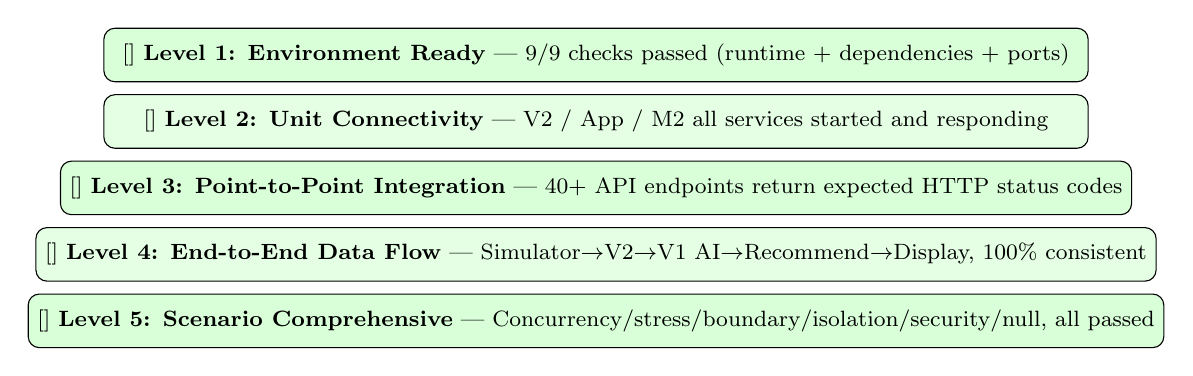
\begin{tikzpicture}[
      level/.style={rectangle,draw,rounded corners,minimum width=12.5cm,minimum height=0.68cm,align=left,font=\footnotesize}]

      \node[level,fill=green!15] (l1) {[\checkmark]\ \textbf{Level 1: Environment Ready} — 9/9 checks passed (runtime + dependencies + ports)};
      \node[level,fill=green!10,below=0.15cm of l1] (l2) {[\checkmark]\ \textbf{Level 2: Unit Connectivity} — V2 / App / M2 all services started and responding};
      \node[level,fill=green!15,below=0.15cm of l2] (l3) {[\checkmark]\ \textbf{Level 3: Point-to-Point Integration} — 40+ API endpoints return expected HTTP status codes};
      \node[level,fill=green!10,below=0.15cm of l3] (l4) {[\checkmark]\ \textbf{Level 4: End-to-End Data Flow} — Simulator$\rightarrow$V2$\rightarrow$V1 AI$\rightarrow$Recommend$\rightarrow$Display, 100\% consistent};
      \node[level,fill=green!15,below=0.15cm of l4] (l5) {[\checkmark]\ \textbf{Level 5: Scenario Comprehensive} — Concurrency/stress/boundary/isolation/security/null, all passed};
    \end{tikzpicture}
  \end{center}
  \vspace{0.1cm}
  \begin{block}{Pending Improvements (Noted, Non-Blocking)}
    \footnotesize
    V2 RBAC access control (Sprint 3)\quad|\quad
    V1 standard curve clinical validation (documented)\quad|\quad
    M2 3D real-time updates (API contract ready)
  \end{block}
\end{frame}

\begin{frame}{Run Guide}
  \begin{block}{One-Click Start All Services}
    \centering
    \texttt{powershell -ExecutionPolicy Bypass -File scripts\textbackslash start\_all.ps1}
  \end{block}

  \begin{block}{Run All Tests in Sequence}
    \centering
    \small
    \begin{tabular}{lcl}
      \toprule
      \textbf{Step} & \textbf{Command} & \textbf{Test Items} \\
      \midrule
      1. Environment Check & \texttt{scripts\textbackslash check\_env.bat} & 9 items \\
      2. Smoke Test & \texttt{...smoke\_test.ps1} & 14 items \\
      3. Full Interface Test & \texttt{...integration\_test.ps1} & 62 items \\
      4. Data Pipeline & \texttt{...pipeline\_test.ps1} & 26 items \\
      5. Scenario \& Stress & \texttt{...scenario\_test.ps1} & 17 items \\
      6. Defect Detection & \texttt{...bug\_hunt.ps1} & 13 items \\
      7. Null Safety & \texttt{...null\_safety.ps1} & 34 items \\
      \bottomrule
    \end{tabular}
  \end{block}

  \begin{center}
    \textbf{Fully automated execution, no manual intervention, 166 total checks}
  \end{center}
\end{frame}

% ============================================================================
\section*{End}
% ============================================================================

\begin{frame}[plain]
  \begin{center}
    \vspace{1.5cm}
    {\LARGE Thank You!}

    \vspace{1cm}
    {\normalsize DSD 2025--2026 \quad UTAD $\times$ Jilin University}

    \vspace{0.5cm}
    {\footnotesize Scripts: \texttt{scripts/} \ | \ Docs: \texttt{TEST\_GUIDE.md} \ | \ PPT: \texttt{docs/integration\_test\_presentation.tex}}
  \end{center}
\end{frame}

\end{document}
